\section{Assignment 4}

\subsection{Compute the dynamic model using the recursive Newton-Euler formulation}

The Newton-Euler formulation is a recursive algorithm used to compute the dynamic model.

\begin{figure}[h]
\centering
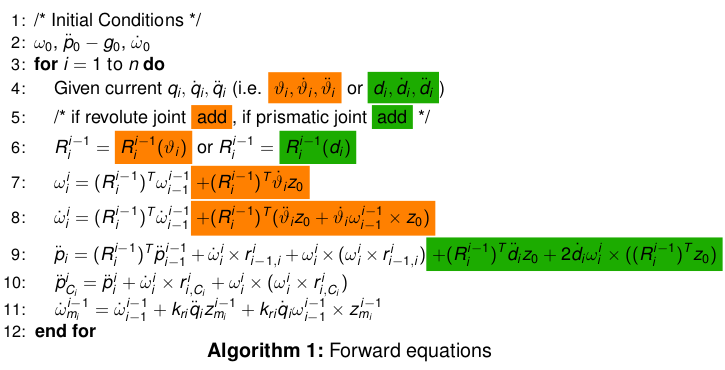
\includegraphics[keepaspectratio,width=0.6\textwidth]{rne_forw}
\end{figure}
\begin{figure}[h]
\centering
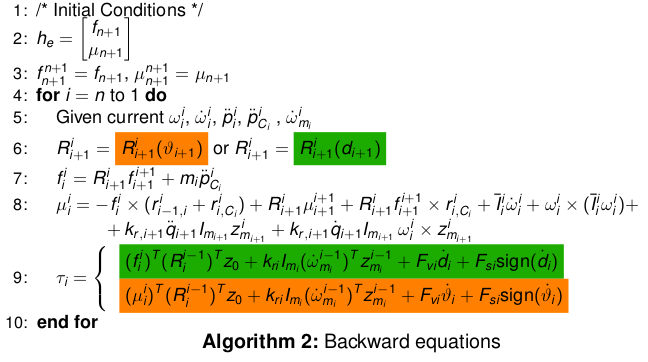
\includegraphics[keepaspectratio,width=0.6\textwidth]{rne_back}
\end{figure}

To check the results, the resulting $B_{RNE}$, $C_{RNE}$ e $g_{RNE}$ were compared to the corresponding quantities computed with the Lagrangian method, in a random robot configuration and joint velocities:

\begin{align*}
B_{RNE} = \begin{bmatrix}
 0.4372& -0.61966  & 0.03208\\
-0.6196&    1.549 &-0.06925\\
 0.03208& -0.069256  &0.04708
\end{bmatrix}&\;\;\;\;\; B_{L} = \begin{bmatrix}
 0.4372& -0.61966   &0.03208\\
-0.6196&    1.549& -0.06925\\
 0.03208& -0.069256 & 0.04708
\end{bmatrix}\\
C_{RNE} = \begin{bmatrix}
 -0.001341\\
0.0005088\\
 -4.893e-5
\end{bmatrix}&\;\;\;\;\; C_{L} = \begin{bmatrix}
 -0.001341\\
  -0.001073\\
0.0002748
\end{bmatrix}\\
g_{RNE} = \begin{bmatrix}
 0\\
  0\\
-0.5539
\end{bmatrix}&\;\;\;\;\; g_{L} = \begin{bmatrix}
0\\
 0\\
-0.5539
\end{bmatrix}\\
\end{align*}
